
Na contemporaneidade, quando se fala de geração de energia, em qualquer local do mundo a primeira questão a ser levantada
é a de maior distribuição possível juntamente com a maior viabilidade econômica envolvida. Estes foram dois parâmetros 
primordiais para se escolher a energia renovável para ser implantada dentro do projeto.

A matriz energética do projeto foi divida em três áreas apresentadas a seguir.

  \subsubsection{Fontes Energéticas Referenciais}
    
    No decorrer do período de elaboração do escopo do projeto, várias possíveis soluções foram levantadas e, em seguida, 
    discutidas com o intuito de se chegar em um sistema que atendesse da melhor formar os requisitos iniciais do projeto.
    Dentre todas as opções disponíveis, foram pré-selecionadas três que, em princípio, se destacaram. São elas:
    
    \begin{itemize}
      \item \textbf{Eole Water}: uma turbina eólica autossuficiente que capta a água a partir de um sistema de refrigeração
	que faz com q a água no ar se condense ao entrar em contato com suas pás \cite{eole}.
     
      \item \textbf{MaxWater}: um moinho de vento vertical, com um sistema muito semelhante ao primeiro, mas que possui custo,
	produção diferenciados.
      
      \item \textbf{Warkawater}:torre feita de bambu e que é forrada por dentro com uma malha plástica, que retém gotículas
	de orvalho. Esse sistema é passivo e não necessita de energia para produção de água já que funciona de forma passiva \cite{warkawater}.
    \end{itemize}
  
    Dois requisitos muitos importantes para a escolha do sistema foram a necessidade do uso de uma fonte energética renovável
    e de que a água fosse analisada em tempo real. Observando o segundo requisito se percebe que existe a necessidade da
    implementação de sensores e de um sistema que envie todos os dados recolhidos por tais sensores. Nesse contexto pensou-se 
    primeiramente no uso de painéis solares fotovoltáicos, em um segundo momento, levando em consideração a região propícia à 
    implementação de um parque eólico e escolha do sistema Eolewater, decidiu-se por utilizar o excedente de energia gerado 
    pela turbina eólica para suprir as necessidades dos sistemas embarcados.
  
    A premissa do uso do potencial dos ventos para geração de trabalho data de milhares de anos atrás, onde essas tecnologias
    eram usadas principalmente para o bombeamento de água e para moagem de grãos. As primeiras tentativas do uso da energia
    eólica para geração de eletricidade foram no século XIX, ma só na década de 1970 é que essa tecnologia foi aplicada em
    escala comercial \cite{cmig}.
    
    A avaliação do potencial eólico de uma região requer trabalhos sistemáticos de coleta e análise de dados sobre a velocidade
    e o regime de ventos. Geralmente, uma avaliação rigorosa requer levantamentos específicos, mas dados coletados em 
    aeroportos, estações meteorológicas e outras aplicações similares podem fornecer uma primeira estimativa do potencial
    bruto ou teórico de aproveitamento da energia eólica \cite{amarante01}.
    
    Embora ainda haja divergências entre especialistas e instituições na estimativa do potencial eólico brasileiro, 
    vários estudos indicam valores extremamente consideráveis. Até poucos anos, as estimativas eram da ordem de 20.000 MW.
    Hoje a maioria dos estudos indica valores maiores que 60.000 MW \cite{amarante01}.
    
    As primeiras turbinas eólicas de uso comercial tinham a capacidade de produção elétrica entre 10kW e 50kW, já
    as máquinas de grande porte atuais tem uma potência superior a 1Mw \cite{dalexandria07}.
    
  \subsubsection{Técnicas e métodos de conversão e armazenamento}
    
    Um dos desafios do projeto foi estabelecer a demanda de água para a região selecionada e a partir disso dimensionar a
    estrutura física necessária de acordo com os requisitos. Dentre os modelos analisados pela equipe, a turbina de vento 
    mais favorável foi a Eolewater, modelo WMS100 Wind Turbine da empresa EoleWater, uma turbina de eixo horizontal que
    apresenta resultados satisfatórios à proposta e servirá de base de estudo para a implementação do projeto na área 
    energética.
    
    Apesar dos avanços nessa área, a energia eólica não possui uma capacidade de produção muito grande, por isso deve-se
    focar no requisito eficiência de conversão. Algumas formas de aperfeiçoar a produção estão relacionadas à dimensão do 
    gerador, aerodinâmica, materiais utilizados, projeção da estrutura e logística.
    
    Partindo dessa necessidade, o gerador exerce função primordial no funcionamento da turbina, pois é ele quem converte a
    energia mecânica em energia elétrica que alimenta todo o sistema. Dessa forma, temos o seguinte esquema de funcionamento:
    Os ventos fazem com que as pás do rotor girem, consequentemente girando o rotor. Este, por sua vez, converte a energia 
    cinética dos ventos em energia mecânica de rotação. Esse conjunto conectado a um eixo transmite essa rotação para o
    gerador. O gerador finalmente converte a energia mecânica em energia elétrica que alimenta todos os outros componentes
    eletrônicos (controle) e mecânicos da turbina.
    
    A produção de energia elétrica estimada da turbina é de aproximadamente 30kW (a produção real depende do diâmetro do rotor,
    rendimento do sistema, velocidade dos ventos, condições climáticas da região). Essa energia produzida alimentará os
    componentes da turbina e a energia remanescente será utilizada pela estação de controle e armazenada em baterias para
    que seja utilizada em situações emergenciais.
    
    Dessa forma, temos a seguinte distribuição energética:
    
    \begin{figure}[!ht]
    \centering
    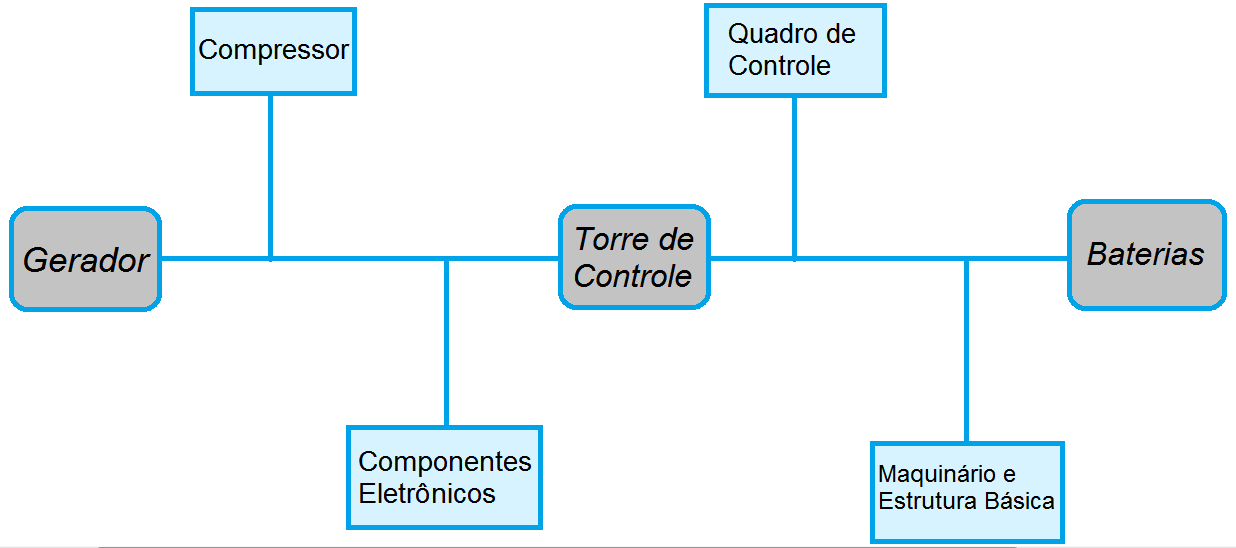
\includegraphics[scale=0.45]{editaveis/figuras/distribuicao_energetica}
    \caption{Distribuição energética}
    \label{distribuicao_energetica}
    \end{figure}
    
    \begin{enumerate}
     \item Geração de eletricidade (aproximadamente 30kW);
     \item Alimentação do compressor e componentes eletrônicos da turbina;
     \item Direcionamento a torre de controle;
     \item Distribuição no quadro de controle;
     \item Alimentação elétrica do maquinário e estrutura básica;
     \item Direcionamento de energia remanescente para as baterias emergenciais.
    \end{enumerate}
    
  \subsubsection{Eficiência Energética}
  
    A turbina eólica, ou aerogerador, é uma máquina capaz de absorver a potência cinética do vento por meio de um rotor
    aerodinâmico, convertendo este movimento em potência mecânica de eixo (torque vs rotação),  que é transformada em
    potência elétrica (tensão \textit{vs} corrente) por intermédio de um gerador elétrico.
    
    A parte estrutural de geração de energia de uma turbina é constituída por um rotor e pela torre que a sustenta,
    pela transmissão/multiplicação e pelo conversor. Ela somente consegue extrair energia através da energia cinética do 
    ar que passa pelo interior da área interceptada pelas pás rotativas.  
    
    O rotor, responsável por transformar a energia cinética em energia mecânica, é o primeiro estágio da conversão.
    Os outros dois são: transmissão mecânica e multiplicação de velocidade; e, por fim, o próprio gerador, responsável
    por converter a energia mecânica em energia elétrica \cite{amaral12}.
    
    Energia eólica provém da radiação solar. Se considerarmos que, aproximadamente, 2\% da energia solar que a Terra absorve,
    é convertida em energia cinética dos ventos, teremos uma estimativa da energia total disponível dos ventos ao redor
    do planeta \cite{terciote02}.
    
    Os ventos (massas de ar em movimento),são influenciados por diferentes aspectos dentre os quais se destacam a rugosidade
    do solo, os obstáculos e o relevo da região, e possuem energia cinética que pode ser aproveitada
    com o uso de aerogeradores \cite{terciote02}.
    
    Dessa forma, a energia cinética $E_C$, contida em uma amostra de volume de ar, $A$ x $\delta x$, com densidade do ar $\rho$, 
    movendo-se com uma velocidade, $v$,  onde $A$ é uma unidade de área perpendicular à direção dos ventos e $\delta x$ é paralelo 
    à direção dos  ventos, é dada por:
    
    O fluxo de massa de ar que penetra as pás do rotor é dada através de  uma amostra de volume de ar, $A$ , com densidade
    do ar $\rho$, movendo-se com uma velocidade, $v$, onde A é uma unidade de área perpendicular à direção dos ventos e $\delta x$
    é paralelo à direção dos  ventos, é dada por:
    
    \begin{figure}[h]
      \begin{center}
	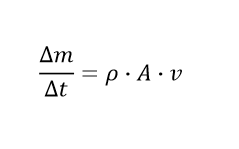
\includegraphics[scale=0.65]{editaveis/figuras/formula_terciote}
	\label{fluxo_ar_pa}
	\caption[Fluxo de ar nas pás do rotor]{Fluxo de ar nas pás do rotor. \footnotemark}
      \end{center}
    \end{figure}
    \FloatBarrier
    \footnotetext{Fonte: \cite{amaral12} }
    
    A primeira vista, imagina-se que a máxima energia retirada dos ventos por uma turbina eólica é a energia cinética dos
    ventos que atravessam um círculo formado pela área das pás. Contudo, o próprio vento possui energia cinética na esteira
    do rotor, fazendo com que nem toda energia seja retirada \cite{terciote02}. Segundo uma teoria criada
    por Betz (1919 \textit{apud} \cite{terciote02})(modelo ideal), a eficiência aerodinâmica do rotos estaria
    limitada a 59,3\% da energia presente nos ventos.
    
    A quantidade de eletricidade que pode ser gerada pelo vento depende de quatro fatores: da quantidade de vento que passa
    pela hélice, do diâmetro da hélice, da dimensão do gerador e do rendimento de todo o sistema \cite{amaral12}.
    
    Em média, a eficiência de conversão dos modernos aerogeradores está dividida
    como ilustra a Figura ~\ref{eficiencia_conversao_aerogeradores}.
    
    \begin{figure}[!ht]
    \centering
    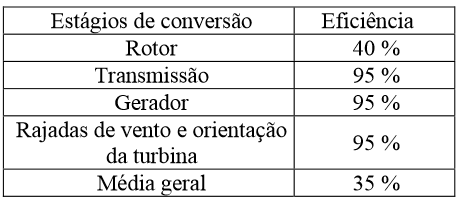
\includegraphics[scale=0.7]{editaveis/figuras/eficiencia_conversao_aerogeradores}
    \caption[Eficiência de conversão dos aerogeradores modernos]{Eficiência de conversão dos aerogeradores modernos. \footnotemark}
    \label{eficiencia_conversao_aerogeradores}
    \end{figure}
    \footnotetext{Fonte: GIPE, 1995 \textit{apud} \cite{terciote02} }
    
    Na contemporaneidade, os parâmetros de rotores utilizados nos aerogeradores modernos são de duas ou três pás.
    Isso graças à relação de potência extraída por área de varredura do rotor (muito superior ao rotor multipás) para 
    velocidades mais elevadas. Tais características são aceitáveis em sistemas de geração de eletricidade, porém se tornam
    inviáveis em sistemas que requeiram altos momentos de força e/ou carga variável \cite{terciote02}.
    
    Rotores modernos, com mais de três pás, são usados somente quando há necessidade de um grande torque de partida, ou seja, 
    basicamente, bombeamento mecânico de água. Aerodinamicamente, no entanto, grande número de pás e alto torque de partida,
    diminuem a eficiência do sistema \cite{terciote02}.

    Sendo assim, o desenvolvimento de pás para aerogeradores deve ser resultante da integração entre estes fatores.
    Com o estágio atual da tecnologia, a dificuldade de fabricação não reside na aerodinâmica, mas sim na construção
    e resistência dos materiais que compõem as pás, que devem responder a diferentes exigências da máquina eólica,
    além de ser necessário que sejam resistentes, rígidos, leves e de baixo custo \cite{terciote02}.
    
    As perdas de transmissão relacionam-se diretamente ao atrito que existe entre as engrenagens.
    Em velocidades de giro fixas, as perdas variam pouco, podendo-se assumir que são uma porcentagem fixa
    da potência nominal. Esta porcentagem real depende da qualidade da transmissão, mas um valor razoável
    pode ser em torno de 2\% da potência em cada etapa de engrenamento. Como a transmissão consome certa quantidade de
    energia, as perdas podem ser consideráveis em baixas potências, já que o rendimento nestes casos é menor
    (JOHANSSON \textit{et al}., 1993 \textit{apud} \cite{terciote02}).
    
    Para que a geração de eletricidade a partir do movimento do ar seja plausível, técnica e economicamente, alguns fatores
    ganham relevância. A velocidade dos ventos é o fator mais crítico na determinação da energia que será obtida de um
    aerogerador, e também seu custo \cite{terciote02}. Segundo \citeauthor{terciote02} (\citeyear{terciote02}), outros fatores seriam:
    \begin{itemize}
     \item \textbf{Topografia}: o ar é mais frio durante a noite e tende a ocupar regiões próximas ao solo, além de produzir
	pouca quantidade de vento. Por isso devem ser escolhidas áreas mais elevadas. Para a escolha dessas áreas devem ser
	observadas também: facilidade de locomoção até a instalação, proximidade ao ponto de consumo, espaço necessário
	para manutenções e evitar áreas muito frias, a fim de não danificar o aerogerador.
	
     \item \textbf{Barreiras Naturais}: prédios, árvores, plantações e construções elevadas que podem diminuir
	a velocidade do vento e turbulência, danificando o equipamento.
      
     \item \textbf{Superfície}: quanto mais acidentado o terreno (maior rugosidade), com plantações, construções, árvores, entre outros,
	mais alta a torre deve ser.
      
     \textit{Obs.:} Quando não especificada a altura na qual ocorreu a medição da velocidade dos ventos,
	consideramos a altura padrão internacional de 10 metros acima do solo, ou a altura em que cada gerador está operando. 
     
    \end{itemize}
    
    O fator de capacidade é uma forma de avaliar o potencial eólico da região, e pode ser interpretado como o percentual 
    de aproveitamento, efetivo ou estimado, do total da potência máxima instalada. Portanto seu cálculo depende das 
    características do aerogerador instalado e das características do local \cite{amaral12}.
    
    Alguns estados do Brasil, como Ceará e Rio Grande do Norte, apresentam um fator de capacidade eólico entre 40\% e 45\%.
    Este é considerado um ótimo resultado, uma vez que, estudos sobre o potencial eólico mostram que a média mundial do fator
    de capacidade é de 27\% \cite{amaral12}.
    
%     Referências não citadas no texto
    \nocite{cbee}